%!TEX TS-program = xelatex
%!TEX encoding = UTF-8 Unicode

\chapter{ข้อมูลสนามบินรายงานต่อฝ่ายข่าวสารการบิน \\
Aerodrome Data for AIS Report}

สนามบินส่วนบุคคล บริเวณขนงพระนี้ เป็น สนามบินสำหรับอากาศยานปีกแข็ง (Fixed-wing Aircraft) 

\section{ข้อมูลทั่วไป (General Information)}

\begin{description}
\item[ชื่อสนามบิน:]  สนามบินขนงพระ
\item[ที่ตั้งสนามบิน:] ตำบลขนงพระ อำเภอปากช่อง จังหวัดนครราชสีมา 30130
\item[ทางภูมิศาสตร์ของจุดอ้างอิงสนามบิน:] Aerodrome Reference Point ที่กำหนดจากฐานอ้างอิงตามระบบ WGS-84 มีรายละเอียดพิกัดและข้อมูล ดังต่อไปนี้

\begin{table}[h]
\caption{Aerodrome Reference Point ที่กำหนดจากฐานอ้างอิงตามระบบ WGS-84}
\begin{center}
\begin{tabular}{|c|c|c|c|c|c|c|c|c|c|}
\hline
\multirow{3}{*}{Point} & \multicolumn{7}{c|}{Geodetic-WGS84 Coordinate} & Elevation & Geoid \\ \cline{2-10}
 & \multicolumn{3}{c|}{Latitude} & \multicolumn{3}{c|}{Longitude} & Ellipsoidal & Height & Undulation \\ \cline{2-10}
  & D & M & S & D & M & S & Height & Above MSL & (N) \\ \hline
  Aerodrome Reference Point & 14 & 37 & 54.48 & 101 & 27 & 52.95 & 321.219 & 349.177 & -27.958 \\
\hline
\end{tabular}
\end{center}
\label{default}
\end{table}%

รายงานการสำรวจ โดยวิศวกรสำรวจ \footnote{ตามแสดงในภาคผนวก ค. (\ref{รายงานการสำรวจสนามบินส่วนบุคคลขนงพระ})}

\item[ระดับความสูงของสนามบิน:]  Aerodrome Elevation และค่าความสูงยีออยด์ (Geoids Undulation)

\begin{table}[h]
\caption{Aerodrome elevation \& Geoids Undulation}
\begin{center}
\begin{tabular}{|c|c|c|c|c|c|c|c|c|c|}
\hline
\multirow{3}{*}{Point} & \multicolumn{7}{c|}{Geodetic-WGS84 Coordinate} & Elevation & Geoid \\ \cline{2-10}
 & \multicolumn{3}{c|}{Latitude} & \multicolumn{3}{c|}{Longitude} & Ellipsoidla & Height & Undulation \\ \cline{2-10}
  & D & M & S & D & M & S & Height & Above MSL & (N) \\ \hline
  Aerodrome Elevation & 14 & 37 & 49.4 & 101 & 28 & 10.7 & 318.457 & 346.393 & -27.936 \\
\hline
\end{tabular}
\end{center}
\label{default}
\end{table}%

\item[ระดับความสูงของหัวทางวิ่ง (Threshold Runway 10) และค่าความสูงยีออยด์ (Geoids Undulation):]  ระดับความสูงของสนามบิน และค่าความสูงยีออยด์ (Geoids Undulation) แต่ละแห่ง ระดับความสูงของปลายทางวิ่ง และจุดที่มีความสูงและต่ำที่สำคัญตามแนวทางวิ่ง

\begin{table}[h]
\caption{ระดับความสูงของหัวทางวิ่ง (Threshold Runway 10) และค่าความสูงยีออยด์ (Geoids Undulation)}
\begin{center}
\begin{tabular}{|c|c|c|c|c|c|c|c|c|}
\hline
\multicolumn{9}{|c|}{\textbf{Coordinates, Elevations \& Geoid Undulation of Runway}} \\ \cline{1-9}
\multirow{3}{*}{Point} & \multicolumn{6}{c|}{Geodetic-WGS84 Coordinate} & Elevation & \multirow{2}{*}{Geoid Undulation} \\ \cline{2-8}
 & \multicolumn{3}{c|}{Latitude} & \multicolumn{3}{c|}{Longitude} & Above & \\ \cline{2-9}
  & D & M & S & D & M & S & MSL Thai & MSL Thai \\ \hline
Threshold Runway 10 & 14 & 37 & 55.40 & 101 & 27 & 45.43 & 342.887 & -27.936 \\
End of Runway & 14 & 37 & 49.38 & 101 & 28 & 10.74 & 346.393 & -27.936 \\
\hline
\end{tabular}
\end{center}
\label{default}
\end{table}%

\item[อุณหภูมิอ้างอิงสนามบิน:] 30 องศา เซลเซียส
\item[รายละเอียดไฟบอกตำแหน่งสนามบิน (Aerodrome Beacon):] ไม่มี
\end{description}

\section{มิติและข้อมูลที่เกี่ยวข้องกับสนามบิน (Aerodrome Dimensions and Related Information)}

\subsection{ทิศจริง และหมายเลขทางวิ่งที่กาหนด ความกว้าง ความยาว ตำแหน่งของหัวทางวิ่งที่เลื่อนไป (Displaced Threshold Runway 10) ความลาดชัน ลักษณะของพื้นผิวและประเภทของทางวิ่ง}

\textbf{ทิศจริง:} วัดที่จุดกึ่งกลางทางวิ่ง (Mid way) จากเมริเดียนจริง (True Meridian) มายังเส้นตรงตามแนวศูนย์กลางหัวท้ายสนามบินเท่ากับ 103 องศา 43 ลิปดา 41.94  ฟิลิปดา  ดังแสดงในตารางข้างล่าง

\begin{table}[h!]
\caption{ทิศจริงของสนามบินส่วนบุคคลขนงพระ}
\begin{center}
\begin{tabular}{|c|c|c|c|c|c|c|c|c|c|c|c|c|}
\hline
\multicolumn{13}{|c|}{\textbf{Azimuth/Bearing of centerline of runway from True North-South}} \\ \hline
\multirow{3}{*}{Point} & \multicolumn{6}{c|}{Geodetic -WGS84 Coordinate} & \multicolumn{3}{c}{Azimuth from} & \multicolumn{3}{c|}{Bearing from} \\ \cline{2-13}
 & \multicolumn{3}{c|}{Latitude} & \multicolumn{3}{c|}{Longitude} & \multicolumn{3}{c|}{True North} & \multicolumn{3}{c|}{True Norht-South} \\ \cline{2-13}
  & D & M & S & D & M & S & D & M & S & D & M & S \\
  \hline
  Threshold Runway 10 & 14 & 37 & 55.4 & 101 & 27 & 45.43 & 103 & 43 & 41.94 & 76 & 16 & 18.06 \\
  End of Runway 28 & 14 & 37 & 49.4 & 101 & 28 & 10.74 & 283 & 43 & 48.09 & 76 & 16 & 11.91 \\
  Mid of Runway & 14 & 37 & 52.39 & 101 & 27 & 58.08 & 103 & 43 & 45.01 & 76 & 16 & 14.99 \\
 \hline

\end{tabular}
\end{center}
\label{default}
\end{table}%

หมายเลขทางวิ่งที่กำหนด ความกว้าง ความยาว ตำแหน่งของหัวทางวิ่งที่เลื่อนไป (Displaced Threshold Runway 10) ความลาดชัน ลักษณะของพื้นผิวและประเภทของทางวิ่ง 

แสดงไว้ในลำดับที่ 1 ของ ตารางที่ \ref{คุณลักษณะโดยรวมของสนามบินส่วนบุคคลขนงพระ} หน้าที่ \pageref{คุณลักษณะโดยรวมของสนามบินส่วนบุคคลขนงพระ}

\subsection{ความกว้าง ความยาว และลักษณะของพื้นผิวของพื้นที่ปลอดภัยรอบทางวิ่ง(Runway Strips) พื้นที่ปลอดภัยปลายทางวิ่ง (Runway End Safety Areas) รวมทั้งของทางหยุด (Stop ways)}

แสดงไว้ในในลำดับที่ 2 ของ ตารางที่ \ref{คุณลักษณะโดยรวมของสนามบินส่วนบุคคลขนงพระ} หน้าที่ \pageref{คุณลักษณะโดยรวมของสนามบินส่วนบุคคลขนงพระ}

\subsection{ความกว้าง ความยาว และลักษณะของพื้นผิวของทางขับ}

แสดงไว้ในในลำดับที่ 3 ของ ตารางที่ \ref{คุณลักษณะโดยรวมของสนามบินส่วนบุคคลขนงพระ} หน้าที่ \pageref{คุณลักษณะโดยรวมของสนามบินส่วนบุคคลขนงพระ}

\subsection{ลักษณะของพื้นผิวลานจอด และหลุมจอดอากาศยาน}

แสดงไว้ในในลำดับที่ 4 ของ ตารางที่ \ref{คุณลักษณะโดยรวมของสนามบินส่วนบุคคลขนงพระ} หน้าที่ \pageref{คุณลักษณะโดยรวมของสนามบินส่วนบุคคลขนงพระ}

\begin{landscape}
\begin{table}[h!]
\caption{คุณลักษณะโดยรวมของสนามบินส่วนบุคคลขนงพระ}
\begin{center}
\begin{tabular}{|c|c|c|c|c|c|c|}
\hline
\textbf{No} & \textbf{Item} & \textbf{Symbol} & \textbf{Width (m)} & \textbf{Length (m)} & \textbf{Surface} & \textbf{Remarks} \\
\hline
\multirow{4}{*}{1} & Runway & - & 20 & 780 & Bitumen & Slope +0.433\% \\ \cline{2-7}
   & Number of Runway: Threshold Runway 10 & 10 & - & - & - & - \\ \cline{2-7}
   & Number of Runway: End & 28 & - & - & - & - \\\cline{2-7}
   & Displaced Threshold Runway 10 & - & - & - & - & -Nil- \\ 
\hline
\multirow{7}{*}{2}  & Runway Strip: Left (A) & - & 9 & 340 & Crushed Rock & - \\ \cline{2-7}
   & Runway Strip Left (B) & - & 18 & 436 & Crushed Rock & - \\ \cline{2-7}
   & Runway Strip Right (A) & - & 14 & 340 & Crushed Rock & - \\ \cline{2-7}
   & Runway Strip Right (B) & - & 21 & 436 & Crushed Rock & - \\ \cline{2-7}
   & Runway End Safety: Threshold Runway 10 & - & 38 & 100 & Bitumen & - \\ \cline{2-7}
   & Runway End Safety: End & - & 40 & 105 & Bitumen & - \\ \cline{2-7}
   & Stopway & - & - & - & - & -Nil - \\ \cline{2-7}
\hline
3   & Taxiway & - & 18 & 8 & Bitumen & - \\
\hline
\multirow{2}{*}{4}   & ลานจอด & 10 & 25 & 56 & Bitumen & - \\ \cline{2-7}
   & ลานจอด & 28 & 128 & 50 & Bitumen & - \\
 \hline 
\end{tabular}
\end{center}
\label{คุณลักษณะโดยรวมของสนามบินส่วนบุคคลขนงพระ}
\end{table}%

\end{landscape}

\subsection{ความกว้าง ความยาว และระดับสูงตำตามแนวยาวของพื้นที่ปลอดสิ่งกีดขวาง (Clearway)}
-ไม่มี-

\subsection{เครื่องช่วยอานวยความสะดวกในการเดินอากาศประเภททัศนวิสัยสาหรับการบินเข้าสู่สนามบินด้วยสายตา (Visual Aids for Approach Procedures)}

\begin{enumerate}
\item Runway Designation Markings 10/28
\item Runway Centerline
\item Wind Sock
\end{enumerate}

เครื่องวัดอากาศ และถุงลม(Wind Direction Indicator) อยู่ในตำแหน่ง ดังแสดงในแผนที และมีพิกัดดังแสดงในตารางที่ \ref{ตำแหน่งเครื่องวัดอากาศและถุงลม} 

\begin{table}[h!]
\caption{ตำแหน่งเครื่องวัดอากาศและถุงลม}
\begin{center}
\begin{tabular}{|c|c|c|c|c|c|c|c|c|}
\hline
\multirow{3}{*}{Point} & \multicolumn{7}{c|}{Geodetic-WGS84 Coordinate} & Elevation \\ \cline{2-9}
 & \multicolumn{3}{c|}{Latitude} & \multicolumn{3}{c|}{Longitude} & Ellipsoidal & Height Above \\ \cline{2-9}
  & D & M & S & D & M & S & Height & MSL Thai \\
\hline
ถุงลม: P1 & 14 & 37 & 53.84 & 101 & 27 & 41.44 & 325.194 & 353.130 \\
ถุงลม: P2 & 14 & 37 & 54.71 & 101 & 27 & 52.44 & 327.445 & 355.381 \\
\hline 
\end{tabular}
\end{center}
\label{ตำแหน่งเครื่องวัดอากาศและถุงลม}
\end{table}%

\subsection{ตำแหน่งและความถี่วิทยุของจุดตรวจสอบคลื่นวิทยุวีโออาร์ (Very High Frequency Aerodrome Checkpoints)}

-ไม่มี-

\subsection{ตำแหน่งและการกำหนดเส้นทางมาตรฐานในการขับเคลื่อน (Standard Taxi Routes)}

-ไม่มี-

\subsection{พิกัดทางภูมิศาสตร์ของหัวทางวิ่งแต่ละด้าน}

ดังแสดงในตาราง \ref{พิกัดทางภูมิศาสตร์ของหัวทางวิ่งแต่ละด้าน}

\begin{table}[h]
\caption{พิกัดทางภูมิศาสตร์ของหัวทางวิ่งแต่ละด้าน}
\begin{center}
\begin{tabular}{|c|c|c|c|c|c|c|c|}
\hline
\multicolumn{8}{|c|}{Coordinates of Runway} \\
\hline
\multirow{3}{*}{Point} & \multicolumn{6}{c|}{Geodetic-WGS84 Coordinate} & \multirow{3}{*}{Distance from Beginning} \\ \cline{2-7}
 & \multicolumn{3}{c|}{Latitude} & \multicolumn{3}{c|}{Longtude} & \\ \cline{2-7}
 & D & M & S & D & M & S & \\
 \hline
 Threshold Runway 10 & 14 & 37 & 55.40 & 101 & 27 & 45.43 & 0.000 \\
 End of Runway & 14 & 37 & 49.38 & 101 & 28 & 10.74 & 780.000 \\
 \hline
\end{tabular}
\end{center}
\label{พิกัดทางภูมิศาสตร์ของหัวทางวิ่งแต่ละด้าน}
\end{table}%

\subsection{พิกัดทางภูมิศาสตร์ของจุดกึ่งกลางทางขับที่เหมาะสม}

จุดกึ่งกลางทางขับที่เหมาะสม อยู่ที่ขอบทางวิ่ง มีพิกัดภูมิศาสตและระดับ 
ดังแสดงในตารางที่ \ref{พิกัดทางภูมิศาสตร์ของจุดกึ่งกลางทางขับที่เหมาะสม}

\begin{table}[h!]
\caption{พิกัดทางภูมิศาสตร์ของจุดกึ่งกลางทางขับที่เหมาะสม}
\begin{center}
\begin{tabular}{|c|c|c|c|c|c|c|c|c|}
\hline
\multirow{3}{*}{Point} & \multicolumn{7}{c|}{Geodetic-WGS84 Coordinate} & Elevation \\ \cline{2-9}
 & \multicolumn{3}{c|}{Latitude} & \multicolumn{3}{c|}{Longitude} & Ellipsoidal & Height Above \\ \cline{2-9}
  & D & M & S & D & M & S & Height & MSL Thai \\
\hline
Taxiway & 14 & 37 & 49.4 & 101 & 28 & 13.98 & 318.4455 & 346.382 \\
\hline 
\end{tabular}
\end{center}
\label{พิกัดทางภูมิศาสตร์ของจุดกึ่งกลางทางขับที่เหมาะสม}
\end{table}%

\subsection{พิกัดทางภูมิศาสตร์ของหลุมจอดอากาศยานแต่ละหลุม}

เนื่องจาก สนามบินส่วนบุคคลขนงพระ เป็นสนามบินแบบ VFR การจอดอากาศยาน จัดระยะห่าง (clearance) ที่ปลอดภัย และ เคลื่อนที่อากาศยานด้วยใช้การเข็น  จึงไม่จำเป็นต้องมีหลุมจอดตายตัว

\subsection{พิกัดทางภูมิศาสตร์และระดับความสูงสุดของสิ่งกีดขวางที่มีผลกระทบต่อการบินในพื้นที่บินเข้าสู่สนามบินและการวิ่งขึ้น ในพื้นที่บินวนและในบริเวณข้างเคียงสนามบิน}

สิ่งกีดขวางที่มีผลกระทบต่อการบินมีพิกัดทางภูมิศาสตร์และระดับความสูงสุด เป็นต้นไม้มีพิกัดทางภูมิศาสตร์และระดับความสูงสุด ดังแสดงในตารางที่ \ref{พิกัดทางภูมิศาสตร์และระดับความสูงสุดของสิ่งกีดขวาง}

\begin{table}[h!]
\caption{พิกัดทางภูมิศาสตร์และระดับความสูงสุดของสิ่งกีดขวาง}
\begin{center}
\begin{tabular}{|c|c|c|c|c|c|c|c|c|}
\hline
\multirow{3}{*}{Point} & \multicolumn{7}{c|}{Geodetic-WGS84 Coordinate} & Elevation \\ \cline{2-9}
 & \multicolumn{3}{c|}{Latitude} & \multicolumn{3}{c|}{Longitude} & Ellipsoidal & Height Above \\ \cline{2-9}
  & D & M & S & D & M & S & Height & MSL Thai \\
\hline
Tree: Highest & 14 & 37 & 47.58 & 101 & 28 & 10.38 & 363.776 & 335.840 \\
Flag Pole: Highest & 14 & 37 & 47.07 & 101 & 28 & 0.85 & 364.299 & 336.363 \\
Electricity Pole: Highest & 14 & 37 & 48.23 & 101 & 28 & 2.84 & 328.700 & 356.636 \\
\hline 
\end{tabular}
\end{center}
\label{พิกัดทางภูมิศาสตร์และระดับความสูงสุดของสิ่งกีดขวาง}
\end{table}%

\newpage

\subsection{ประเภทของผิวพื้นจราจร และการรับน้ำหนักของผิวพื้นจราจร}

ผิวพื้นทางวิ่งและทางขับของสนามบินขนงพระถูกออกแบบเพื่อให้สามารถรองรับน้ำหนักบรรรทุกเฉลี่ย 30ตัน
รายงานการเจาะสำรวจ และการรับรองการรับน้ำหนักอากาศยานโดยวิศวกร ตามเอกสารรายละเอีดยการคำนวนและรับรองโดยวิศวกรวิชาชีพ \footnote{รายละเอียดการออกแบบ และ Drawings ใน ผนวก ง. \ref{ข้อมูลรายละเอียด Runway ของสนามบินส่วนบุคคลขนงพระ}}

\subsection{ที่ตั้งของจุดตรวจสอบเครื่องวัดความสูงของอากาศยาน (Altimeter)}

ที่ตั้งของจุดตรวจสอบเครื่องวัดความสูงของอากาศยาน (Altimeter) อยู่ที่ศูนย์กลางลานจอดมีพิกัดทางภูมิศาสตร์และระดับความสูง ดังแสดงในตารางที่ \ref{ที่ตั้งของจุดตรวจสอบเครื่องวัดความสูงของอากาศยาน (Altimeter)}

\begin{table}[h!]
\caption{ที่ตั้งของจุดตรวจสอบเครื่องวัดความสูงของอากาศยาน (Altimeter)}
\begin{center}
\begin{tabular}{|c|c|c|c|c|c|c|c|c|}
\hline
\multirow{3}{*}{Point} & \multicolumn{7}{c|}{Geodetic-WGS84 Coordinate} & Elevation \\ \cline{2-9}
 & \multicolumn{3}{c|}{Latitude} & \multicolumn{3}{c|}{Longitude} & Ellipsoidal & Height Above \\ \cline{2-9}
  & D & M & S & D & M & S & Height & MSL Thai \\
\hline
ลานจอด 10 & 14 & 37 & 55.75 & 101 & 27 & 41.59 & 314.949 & 342.885 \\
ลานจอด 28 & 14 & 37 & 50.57 & 101 & 28 & 13.65 & 318.443 & 346.379 \\
\hline 
\end{tabular}
\end{center}
\label{ที่ตั้งของจุดตรวจสอบเครื่องวัดความสูงของอากาศยาน (Altimeter)}
\end{table}%

\subsection{ความยาว TORA TODA  ASDA และ LDA}

\begin{table}[h!]
\caption{ข้อมูลความยาว TORA TODA  ASDA และ LDA}
\begin{center}
\begin{tabular}{|c|c|c|c|c|}
\hline
Runway & TORA (m) & TODA (m) & ASDA (m) & LDA (m) \\
\hline
10 & 780 & 780 & 780 & 780 \\
28 & 780 & 780 & 780 & 780 \\
\hline
\end{tabular}
\end{center}
\label{ข้อมูลความยาว TORA TODA  ASDA และ LDA}
\end{table}%

\subsection{แผนการเคลื่อนย้ายอากาศยานขัดข้องและข้อมูลเกี่ยวกับความสามารถในการเคลื่อนย้ายอากาศยานขัดข้อง}

สนามบินขนงพระ เป็นสนามบินส่วนบุคคล รองรับอากาศยานขนาดเล็ก หากเกิดกรณีมีอากาศยานขัดข้องบนทางวิ่ง สนามบินขนงพระจะปิดการให้บริการ และเนื่องจากอากาศยานที่จะสามารถบินขึ้นลง บนทางวิ่งขนาด 780 เมตรได้ ต้องเป็นอากาศยานขนาดเล็ก การเคลื่อนย้ายอากาศยานออกนอกทางวิ่งทำโดยการใช้กำลังคนและรถยนต์และรถแทรกเตอร์ของสนามบินในการเคลื่อนย้าย

การแจ้งเหตุเป็นไปตาม แผนฉุกเฉินของสนามบินส่วนบุคคล (Aerodrome Emergency Program) โดยมี เบอร์โทรศัพท์ติดต่อกรณีฉุกเฉินสนามบิน ดังต่อไปนี้

\begin{enumerate}
\item ผู้จัดการสนามบิน 086 657 1510
\item ผู้ช่วยผู้จัดการสนามบิน 089 478 0808
\item สถานีตำรวจภูธรหนองสาหร่าย
	\begin{description}
		\item[มือถือ] 082-1506642
		\item[โทรศัพท์/แฟ็กซ์] 044-938794 และ 044-938795
\end{description}
\item โรงพยายาลกรุงเทพปากช่อง 044-316611-5
\end{enumerate}

\subsection{การกู้ภัยและดับเพลิง (Rescue and Fire Fighting)}

สนามบินขนงพระ มีขีดความสามารถในการดับเพลิงและกู้ภัยสนามบินระดับ 1 (Category 1) โดยมี ถังดับเพลิง จำนวน 6 ถัง ชนิดผงเคมีแห้ง ขนาด 15 กิโลกรัม

\begin{figure}[h!]
\begin{center}
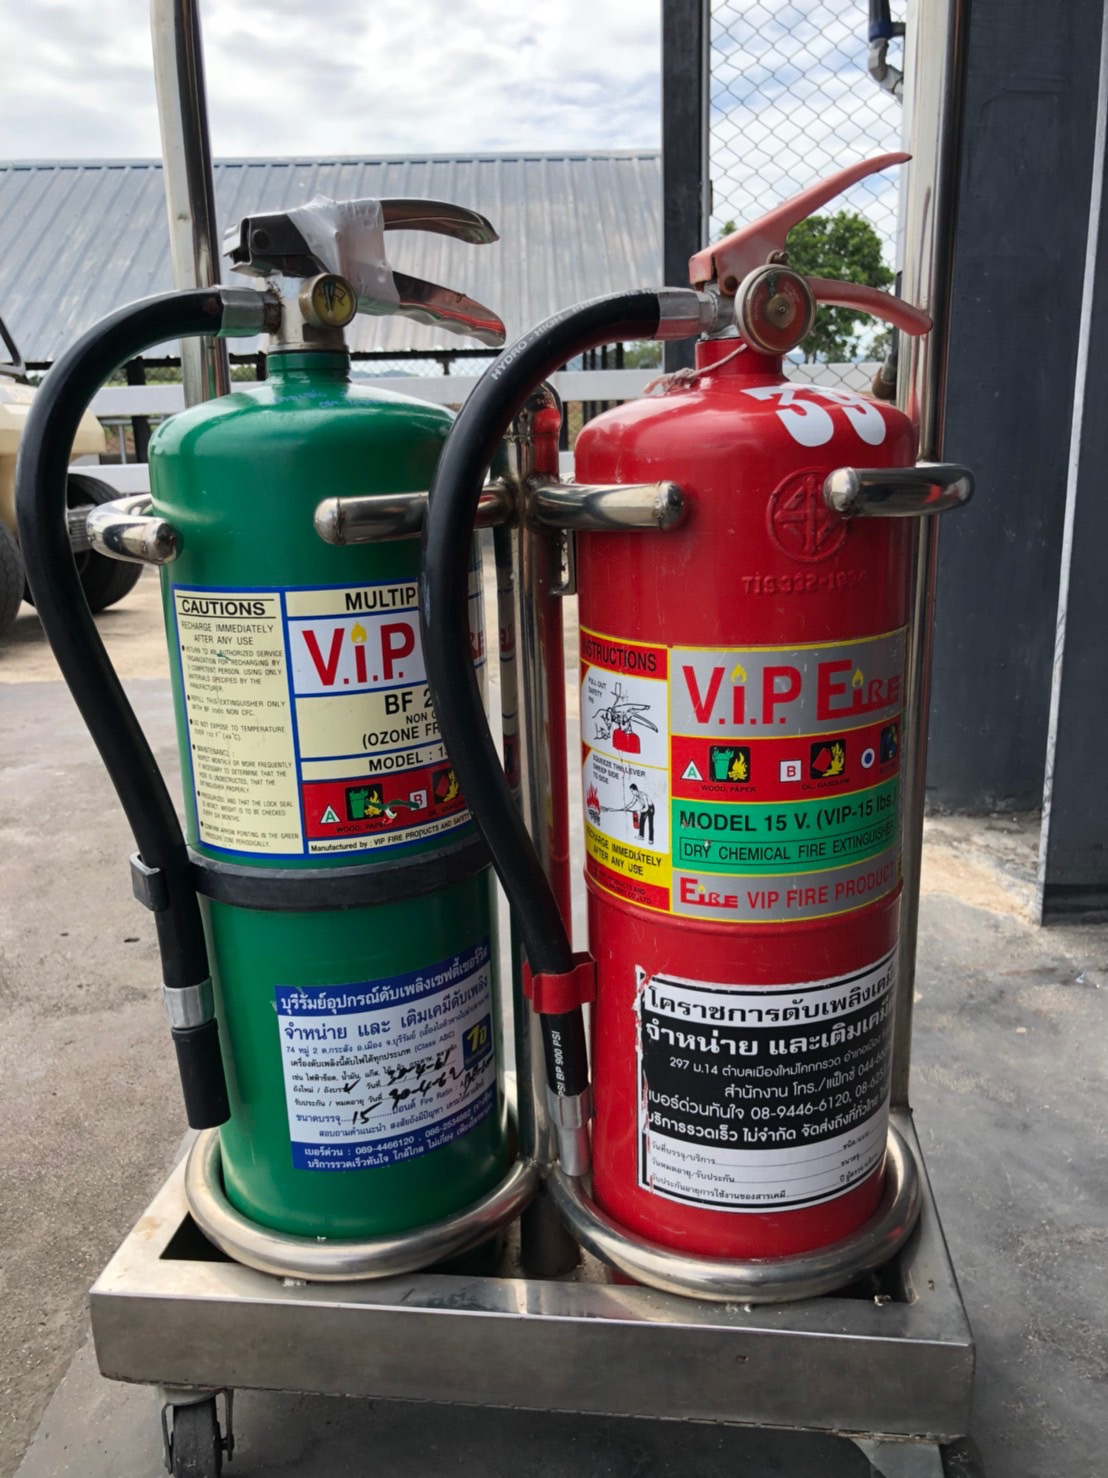
\includegraphics[width=0.4\linewidth]{images/Fire_Extinguisher.jpg}
\caption{ตัวอย่างถังดับเพลิงประจำสนามบินส่วนบุคคลขนงพระ}
\label{ตัวอย่างถังดับเพลิงประจำสนามบินส่วนบุคคลขนงพระ}
\end{center}
\end{figure}
